\section{2022/2/22}

基础知识
\subsection{空间理论}

$C([a,b])$
\par
$L^p(\Omega)\, (\Omega,\Sigma,\mu)$
\par
H{\"o}lder,Minkowski Inequality
\par
\subsubsection{弱$L^p$空间}
\par
{\bfseries 定义:}设$f\in \mathcal{M}(\Omega)$,且$\alpha\in[0,+\infty)$,令$d_f(\alpha)=\mu\{x\in\Omega\big| |f(x)|>\alpha\}$,称$d_f$为$f$的分布函数。
\par
{\bfseries 性质:}
\begin{itemize}
    \item $d_f(\alpha)$关于$\alpha$单调递减。
    \item 右连续。
\end{itemize}

{\bfseries 定理:}设$0<p<\infty$,$f\in L^p$,则有:
\begin{equation*}
    \int_{\Omega}|f(x)|^p\dd x=\int_0^{+\infty}p\alpha^{p-1}d_f(\alpha)\dd \alpha
\end{equation*}

\begin{proof}
    \begin{equation*}
        \begin{aligned}
            \int_{\Omega}|f(x)|^p\dd x&=\int_{\Omega}\int_{0}^{|f(x)|}\frac{1}{p}\alpha^{p-1}\dd \alpha \dd x\\
            &=\int_{\Omega}\int_{0}^{\infty}\frac{1}{p}\alpha^{p-1}\chi_{0<\alpha<|f(x)|}\dd \alpha \dd x\\
            &=\int_{0}^{\infty}\frac{1}{p}\alpha^{p-1}\int_{\Omega}\chi_{0<\alpha<|f(x)|}\dd x\dd \alpha \\
            &=\int_{0}^{\infty}\frac{1}{p}\alpha^{p-1}d_f(\alpha)\dd \alpha
        \end{aligned}
    \end{equation*}
\end{proof}

{\bfseries\large 定义:}设$(\Omega,\sum,\mu)$ , $0<p<\infty$ . $f\in\mathcal{M}(\Omega)$ , 令:
\begin{equation*}
    \begin{aligned}
        \norm*{f}_{L^{p,\infty}}&=\sup_{\alpha>0}\alpha d_f^{\frac{1}{p}}(\alpha)\\
        &=\inf\{ C>0:\alpha d_{f}^{\frac{1}{p}}(\alpha)\leq C,\forall \alpha>0 \}
    \end{aligned}
\end{equation*}
令$L^{p,\infty}$由所有的$\norm*{f}_{L^{p,\infty}}<\infty$的函数构成,并称$L^{p,\infty}(\Omega)$为弱$L^p$空间。
\\
$p=\infty$,令$L^{\infty,\infty}=L^{\infty}$。且$\norm*{f}_{L^{\infty,\infty}}=\norm*{f}_{L^{\infty}}$。
\\
{\bfseries \large 注:}$L^{p,\infty}$是向量空间,且是拟赋范的(且完备)
\\
范数:$\norm*{f+g}\leq \norm*{f}+\norm*{g}$\\
拟范数:$\norm*{f+g}\leq K(\norm*{f}+\norm*{g}),K\geq 1$
\\
\begin{proof}
    \begin{equation*}
        \begin{aligned}
            d_{f+g}(\alpha)&=\mu(|f+g|>\alpha)\\
            &\leq \mu(|f|+|g|>\alpha)\\
            &\leq \mu(|f|>\frac{\alpha}{2})+\mu(|g|>\frac{\alpha}{2})
        \end{aligned}
    \end{equation*}
    若$P>1$,则得
    \begin{equation*}
        \begin{aligned}
            \alpha d_{f+g}^{\frac{1}{p}}(\alpha)
            &\leq \alpha(d_f(\frac{\alpha}{2})+d_g(\frac{\alpha}{2}))^{\frac{1}{p}}\\ &\leq 2\left(\frac{\alpha}{2}d_f^{\frac{1}{p}}(\frac{\alpha}{2})+\frac{\alpha}{2}d_g^{\frac{1}{p}}(\frac{\alpha}{2})\right)
        \end{aligned}
    \end{equation*}
    即
    \begin{equation*}
        \norm*{f+g}_{L^{p,\infty}}\leq 2(\norm*{f}_{L^{p,\infty}} + \norm*{g}_{L^{p,\infty}} )
    \end{equation*}
\end{proof}

{\bfseries \large 定理:}$0<p\leq \infty$,有$L^p\subset L^{p,\infty}$。
\begin{proof}
    任取$f\in L^p$,有:
    \begin{equation*}
        \begin{aligned}
         \alpha^p d_f{\alpha}&=\alpha^p \mu(|f|\geq \alpha)\\
         &=\alpha^p\int_{(|f(x)|>\alpha)}1\dd x\\
         &\leq \int_{(|f|>\alpha)}|f(x)|^p\dd x\\
         &\leq \int_{\Omega}|f(x)|^p\dd x<\infty 
        \end{aligned}
    \end{equation*}
\end{proof}

$f_n\xrightarrow{L^p}f\Rightarrow f_n\xrightarrow{L^{p,\infty}}f\Rightarrow f_n\xrightarrow{\mu}f$
\\
{\bfseries \large 例:(Littlewood's Inequality)}$f\in L^p\cap L^r$ , $0<p<q<r\leq \infty$ , $\frac{1}{q}=\frac{\theta}{p}+\frac{1-\theta}{r},\quad 0<\theta<1$ 则$f\in L^q$ ,且满足
\begin{equation*}
    \norm*{f}_{L^q}\leq \norm*{f}_{L^p}^{\theta}\norm*{f}_{L^r}^{1-\theta}
\end{equation*}
\begin{proof}
    $0<p<q<r\leq \infty$ , $\frac{1}{q}=\frac{\theta}{p}+\frac{1-\theta}{r},\quad 0<\theta<1$ , 再利用H{\"o}lder不等式证明即可。
    \\
    \begin{equation*}
        \begin{aligned}
            \norm*{f}_{L^q}&=(\int|f|^q)^{\frac{1}{q}}\\
            & =(\int |f|^{\theta q+(1-\theta)q})^{\frac{1}{q}}\\
            & \leq \left((\int|f|^{\theta q \frac{p}{\theta q}})^{\frac{\theta q}{p}} (\int|f|^{(1-\theta) q \frac{r}{(1-\theta)q}})^{\frac{(1-\theta) q}{r}}\right)^{\frac{1}{q}}\\
            &\leq  (\int |f|^p)^{\frac{\theta}{p}} (\int |f|^r)^{\frac{1-\theta}{r}}=\norm*{f}_{L^p}^{\theta}\norm*{f}_{L^r}^{1-\theta} <\infty
        \end{aligned}
    \end{equation*}
    再证$r=\infty$的情况:
    \begin{equation*}
        (\int|f|^q)^{\frac{1}{q}}=(\int|f|^{\frac{p}{\theta}})^{\frac{\theta}{p}}\leq (\int|f|^p)^{\frac{\theta}{p}}(\norm*{f}_{L^{\infty}}^{\frac{p}{\theta}-p})^{\frac{\theta}{p}}=\norm*{f}_{L^p}^{\theta}\norm*{f}_{L^\infty}^{1-\theta}
    \end{equation*}
\end{proof}

{\bfseries \large 定理:(Interpolation)}设$0<p<q<r\leq \infty$,$\frac{1}{q}=\frac{1-\theta}{p}+\frac{\theta}{r}$,若$f\in L^{p,\infty}\cap L^{r,\infty}$。则$f\in L^q$且$\norm*{f}_{L^q}\leq \norm*{f}_{L^{p,\infty}}^{1-\theta}\norm*{f}_{L^{r,\infty}}^{\theta}$

\begin{proof}
    
\end{proof}

\begin{itemize}
    \item Lipschitz空间
    \item H{\"o}lder空间
    \item $C^k([a,b])$ , $\norm*{f}_{\infty}=\sup_{x\in[a,b]}\abs*{f(x)}$ ,该范数下不是Banach空间。\\$\sup\sum_{|m|\leq k}\abs*{f^{(m)}(x)}$
    \item $C_0^{\infty}(\mathbb{R}^n)$ , $C^{\infty}(\mathbb{R}^n)$ , $S\subset(\mathbb{R}^n)$
    \item Sobolev空间
    \item Lorentz空间\\
    $\norm*{f}_{L^p}=(\int|f|^p)^{\frac{1}{p}}=(\int_0^{+\infty}p\alpha^{p-1}d_f(\alpha)\dd \alpha)^{\frac{1}{p}}=p^{\frac{1}{p}}\left(\int_0^{+\infty} (\alpha d_f^{\frac{1}{p}}(\alpha))^p \frac{\dd \alpha}{\alpha} \right)^{\frac{1}{p}}$\\
    $\norm*{f}_{L^{p,\infty}}=\sup_{\alpha>0}\alpha d_f^{\frac{1}{p}}(\alpha)$\\
    $\norm*{f}_{L^{p,q}}=p^{\frac{1}{q}}\left(\int_0^{+\infty} (\alpha d_f^{\frac{1}{p}}(\alpha))^q \frac{\dd \alpha}{\alpha} \right)^{\frac{1}{q}}$=$\norm*{\alpha d_f^{\frac{1}{p}}(\alpha)}_{L(R^+,\frac{\dd \alpha}{\alpha})}$
\end{itemize}

{\bfseries \large 例:}$L^p\subset L^{p,\infty}$ , 但是不一定有$L^p\supset L^{p,\infty}$.
\\
$f(x)=\frac{1}{x},\quad x\in (0,+\infty)$ , $f\in L^{1,\infty}(0,\infty)$ , $f\not\in L^1(0,\infty)$。

\subsection{局部紧群与卷积}

{\bfseries \large 定义:} $G$是群且$G$是局部紧拓扑空间,且两个结构相容(逆运算与乘法运算均连续)
\\
{\bfseries \large 命题:}
设$G$是局部紧群,则$G$上存在一个正则的Borel测度,$\mu$且$\mu$是左不变的。即$\forall A$为开集,$\forall \lambda\in G$,有:
\begin{equation*}
    \mu(\lambda A)=\mu A
\end{equation*}
称为左不变Haar测度。
\begin{proof}
    
\end{proof}

{\bfseries \large 例1:}$(R^n,+)$ , $\mu(x,+A)=\mu A$。

{\bfseries \large 例2:}$I=(0,+\infty)$ \\
通常拓扑:
\begin{equation*}
    \int_0^{+\infty}f(x)\frac{\dd x}{x}
\end{equation*}
$\forall x\in I$ , $\int_0^{+\infty}f(\lambda x)\frac{\dd x}{x}=\int_0^{+\infty}f(x)\frac{\dd x}{x}$ . 
\\
对应的测度为$\frac{\dd x}{x}$. $f\in L^1(\frac{\dd x}{x})$ , $\norm*{f}_{L^1(I,\frac{\dd x}{x})}=\int_0^{+\infty}f(x)\frac{\dd x}{x}$。\\
{\bfseries \large 例3:}$L^1(\Pi)$ , $\Pi=R/Z$ , $\Pi^n=R^n/Z^n$,\\
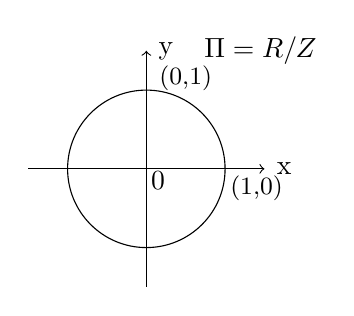
\begin{tikzpicture}
    \draw [->] (0,1.5)--(3,1.5);
    \draw [->] (1.5,0)--(1.5,3);
    \draw [->] (1.5,1.5) circle (1);
    \draw (1.65,1.35) node {0};
    \draw (1.75,3) node {y};
    \draw (3.25,1.5) node {x};
    \draw (2.9,1.25) node{\small(1,0)};
    \draw (2,2.65) node {\small(0,1)};
    \draw (2.95,3) node {$\Pi=R/Z$};
\end{tikzpicture}
$\int_{\Pi}f(x+t)\dd t=\int_{\Pi}f(t)\dd t$
\\
{\bfseries \large 定义:}设$G$为局部紧群。$f,g\in L^1(G)$,即称
\begin{equation*}
    f\star g(x)=\int_{G}f(y)g(y^{-1}x)\dd y
\end{equation*}
为$f$与$g$的卷积。
\\
{\bfseries \large 注:}
\begin{equation*}
    \begin{aligned}
        \norm*{f\star g}_{L^1}&=\int_{G}|\int_{G}f(y)g(y^{-1}x)\dd y|\dd x\\
        &=\int_{G}\int_G \abs*{f(y)g(y^{-1}x)}\dd x\dd y\\
        &=\int_G\abs*{f(y)}\dd y\cdot \int_G\abs*{g(x)}\dd x\,\,(\int_G\abs*{g(x)}\dd x<\infty)
    \end{aligned}
\end{equation*}

{\bfseries \large 注:}
\begin{equation*}
    \star\, f\mapsto f\star g, L^1\rightarrow L^1
\end{equation*}
即$\star\in B(L^1)$.
\\
{\bfseries \large 定理(Young):}设$f\in L^p(R^n)$ , $g\in L^1(\mathbb{R}^n)$ , $1\leq p\leq \infty$ ,则$g\star f\in L^p(R^n)$ 且 $\norm*{g\star f}_{L^p}\leq \norm*{f}_{L^p}\norm*{g}_{L^1}$.
\\
{\bfseries \large 定理(Young):} $1\leq p,q,r\leq\infty$,且$\frac{1}{q}+1=\frac{1}{p}+\frac{1}{r}$,若$f\in L^p(R^n)$ , $g\in L^r(R^n)$ ,则$f\star g\in L^q(R^n)$且
\begin{equation*}
    \norm*{f\star g}_{L^q}\leq \norm*{f}_{L^p}\norm*{g}_{L^r}
\end{equation*}
\\
{\bfseries \large 定理(弱Young):}
以上三个定理的叙述及证明可见《Classical fourier analysis》 Grafakos ,  Loukas.P22